\documentclass[man]{apa6}
\usepackage{lmodern}
\usepackage{amssymb,amsmath}
\usepackage{ifxetex,ifluatex}
\usepackage{fixltx2e} % provides \textsubscript
\ifnum 0\ifxetex 1\fi\ifluatex 1\fi=0 % if pdftex
  \usepackage[T1]{fontenc}
  \usepackage[utf8]{inputenc}
\else % if luatex or xelatex
  \ifxetex
    \usepackage{mathspec}
  \else
    \usepackage{fontspec}
  \fi
  \defaultfontfeatures{Ligatures=TeX,Scale=MatchLowercase}
\fi
% use upquote if available, for straight quotes in verbatim environments
\IfFileExists{upquote.sty}{\usepackage{upquote}}{}
% use microtype if available
\IfFileExists{microtype.sty}{%
\usepackage{microtype}
\UseMicrotypeSet[protrusion]{basicmath} % disable protrusion for tt fonts
}{}
\usepackage{hyperref}
\hypersetup{unicode=true,
            pdftitle={The title},
            pdfauthor={First Author~\& Ernst-August Doelle},
            pdfkeywords={keywords},
            pdfborder={0 0 0},
            breaklinks=true}
\urlstyle{same}  % don't use monospace font for urls
\usepackage{graphicx,grffile}
\makeatletter
\def\maxwidth{\ifdim\Gin@nat@width>\linewidth\linewidth\else\Gin@nat@width\fi}
\def\maxheight{\ifdim\Gin@nat@height>\textheight\textheight\else\Gin@nat@height\fi}
\makeatother
% Scale images if necessary, so that they will not overflow the page
% margins by default, and it is still possible to overwrite the defaults
% using explicit options in \includegraphics[width, height, ...]{}
\setkeys{Gin}{width=\maxwidth,height=\maxheight,keepaspectratio}
\IfFileExists{parskip.sty}{%
\usepackage{parskip}
}{% else
\setlength{\parindent}{0pt}
\setlength{\parskip}{6pt plus 2pt minus 1pt}
}
\setlength{\emergencystretch}{3em}  % prevent overfull lines
\providecommand{\tightlist}{%
  \setlength{\itemsep}{0pt}\setlength{\parskip}{0pt}}
\setcounter{secnumdepth}{0}
% Redefines (sub)paragraphs to behave more like sections
\ifx\paragraph\undefined\else
\let\oldparagraph\paragraph
\renewcommand{\paragraph}[1]{\oldparagraph{#1}\mbox{}}
\fi
\ifx\subparagraph\undefined\else
\let\oldsubparagraph\subparagraph
\renewcommand{\subparagraph}[1]{\oldsubparagraph{#1}\mbox{}}
\fi

%%% Use protect on footnotes to avoid problems with footnotes in titles
\let\rmarkdownfootnote\footnote%
\def\footnote{\protect\rmarkdownfootnote}


  \title{The title}
    \author{First Author\textsuperscript{1}~\& Ernst-August
Doelle\textsuperscript{1,2}}
    \date{}
  
\shorttitle{Title}
\affiliation{
\vspace{0.5cm}
\textsuperscript{1} Wilhelm-Wundt-University\\\textsuperscript{2} Konstanz Business School}
\keywords{keywords\newline\indent Word count: X}
\usepackage{csquotes}
\usepackage{upgreek}
\captionsetup{font=singlespacing,justification=justified}

\usepackage{longtable}
\usepackage{lscape}
\usepackage{multirow}
\usepackage{tabularx}
\usepackage[flushleft]{threeparttable}
\usepackage{threeparttablex}

\newenvironment{lltable}{\begin{landscape}\begin{center}\begin{ThreePartTable}}{\end{ThreePartTable}\end{center}\end{landscape}}

\makeatletter
\newcommand\LastLTentrywidth{1em}
\newlength\longtablewidth
\setlength{\longtablewidth}{1in}
\newcommand{\getlongtablewidth}{\begingroup \ifcsname LT@\roman{LT@tables}\endcsname \global\longtablewidth=0pt \renewcommand{\LT@entry}[2]{\global\advance\longtablewidth by ##2\relax\gdef\LastLTentrywidth{##2}}\@nameuse{LT@\roman{LT@tables}} \fi \endgroup}


\DeclareDelayedFloatFlavor{ThreePartTable}{table}
\DeclareDelayedFloatFlavor{lltable}{table}
\DeclareDelayedFloatFlavor*{longtable}{table}
\makeatletter
\renewcommand{\efloat@iwrite}[1]{\immediate\expandafter\protected@write\csname efloat@post#1\endcsname{}}
\makeatother
\usepackage{lineno}

\linenumbers

\authornote{Add complete departmental affiliations for each
author here. Each new line herein must be indented, like this line.
Enter author note here.

Correspondence concerning this article should be addressed to First
Author, Postal address. E-mail:
\href{mailto:my@email.com}{\nolinkurl{my@email.com}}}

\abstract{
One or two sentences providing a \textbf{basic introduction} to the
field, comprehensible to a scientist in any discipline.

Two to three sentences of \textbf{more detailed background},
comprehensible to scientists in related disciplines.

One sentence clearly stating the \textbf{general problem} being
addressed by this particular study.

One sentence summarizing the main result (with the words ``\textbf{here
we show}'' or their equivalent).

Two or three sentences explaining what the \textbf{main result} reveals
in direct comparison to what was thought to be the case previously, or
how the main result adds to previous knowledge.

One or two sentences to put the results into a more \textbf{general
context}.

Two or three sentences to provide a \textbf{broader perspective},
readily comprehensible to a scientist in any discipline.


}

\begin{document}
\maketitle

\begin{verbatim}
## # A tibble: 6 x 13
##   school_id urban level minority enroll tt_cm tt_dp tt_s  tt_wsvb tt_pbi
##       <dbl> <chr> <chr> <chr>    <chr>  <chr> <chr> <chr> <chr>   <chr> 
## 1         3 Urba~ Midd~ 20 to 5~ Less ~ yes   yes   yes   yes     yes   
## 2         3 Urba~ Midd~ 20 to 5~ Less ~ yes   yes   yes   yes     yes   
## 3         3 Urba~ Midd~ 20 to 5~ Less ~ yes   yes   yes   yes     yes   
## 4         4 Town  Prim~ 50 perc~ 500-9~ yes   yes   yes   no      yes   
## 5         4 Town  Prim~ 50 perc~ 500-9~ yes   yes   yes   no      yes   
## 6         4 Town  Prim~ 50 perc~ 500-9~ yes   yes   yes   no      yes   
## # ... with 3 more variables: oss <dbl>, discipline_type <chr>,
## #   frequency <dbl>
\end{verbatim}

\begin{verbatim}
## # A tibble: 6 x 13
##   school_id urban level minority enroll tt_cm tt_dp tt_s  tt_wsvb tt_pbi
##       <dbl> <chr> <chr> <chr>    <chr>  <chr> <chr> <chr> <chr>   <chr> 
## 1         3 Urba~ Midd~ 20 to 5~ Less ~ yes   yes   yes   yes     yes   
## 2         3 Urba~ Midd~ 20 to 5~ Less ~ yes   yes   yes   yes     yes   
## 3         3 Urba~ Midd~ 20 to 5~ Less ~ yes   yes   yes   yes     yes   
## 4         4 Town  Prim~ 50 perc~ 500-9~ yes   yes   yes   no      yes   
## 5         4 Town  Prim~ 50 perc~ 500-9~ yes   yes   yes   no      yes   
## 6         4 Town  Prim~ 50 perc~ 500-9~ yes   yes   yes   no      yes   
## # ... with 3 more variables: oss <dbl>, discipline_type <fct>,
## #   frequency <dbl>
\end{verbatim}

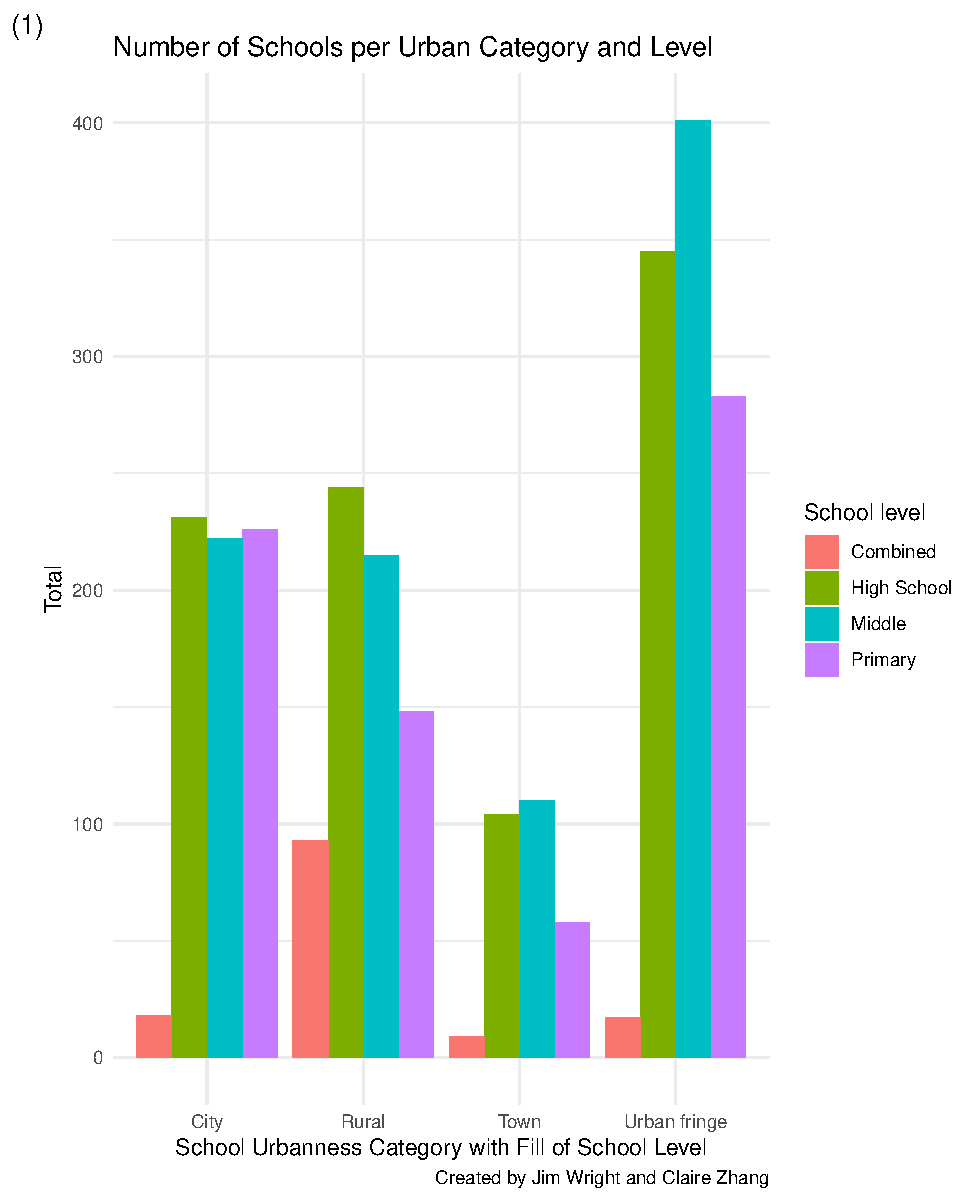
\includegraphics{Final-Project_Zhang_Wright_files/figure-latex/plots-1.pdf}
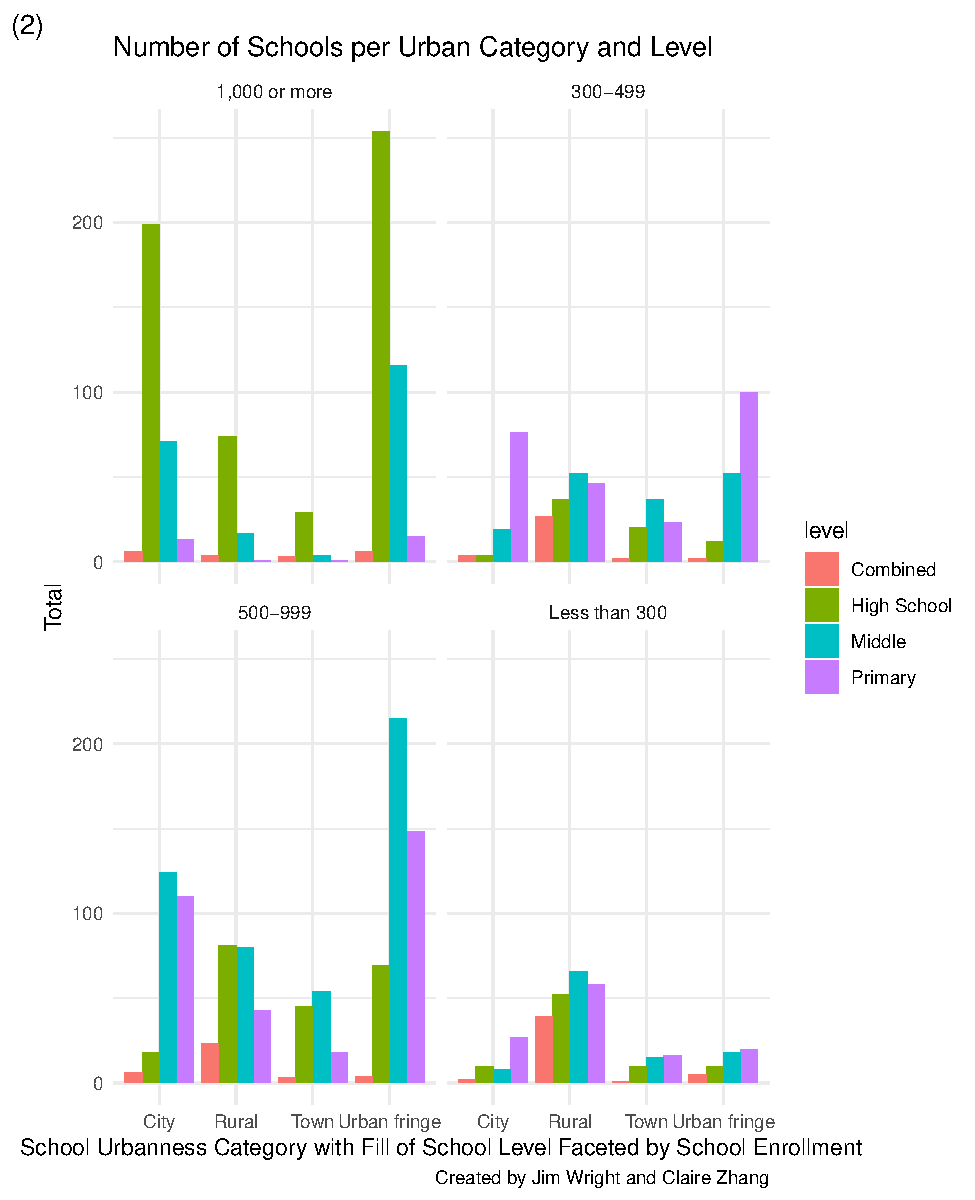
\includegraphics{Final-Project_Zhang_Wright_files/figure-latex/plots-2.pdf}
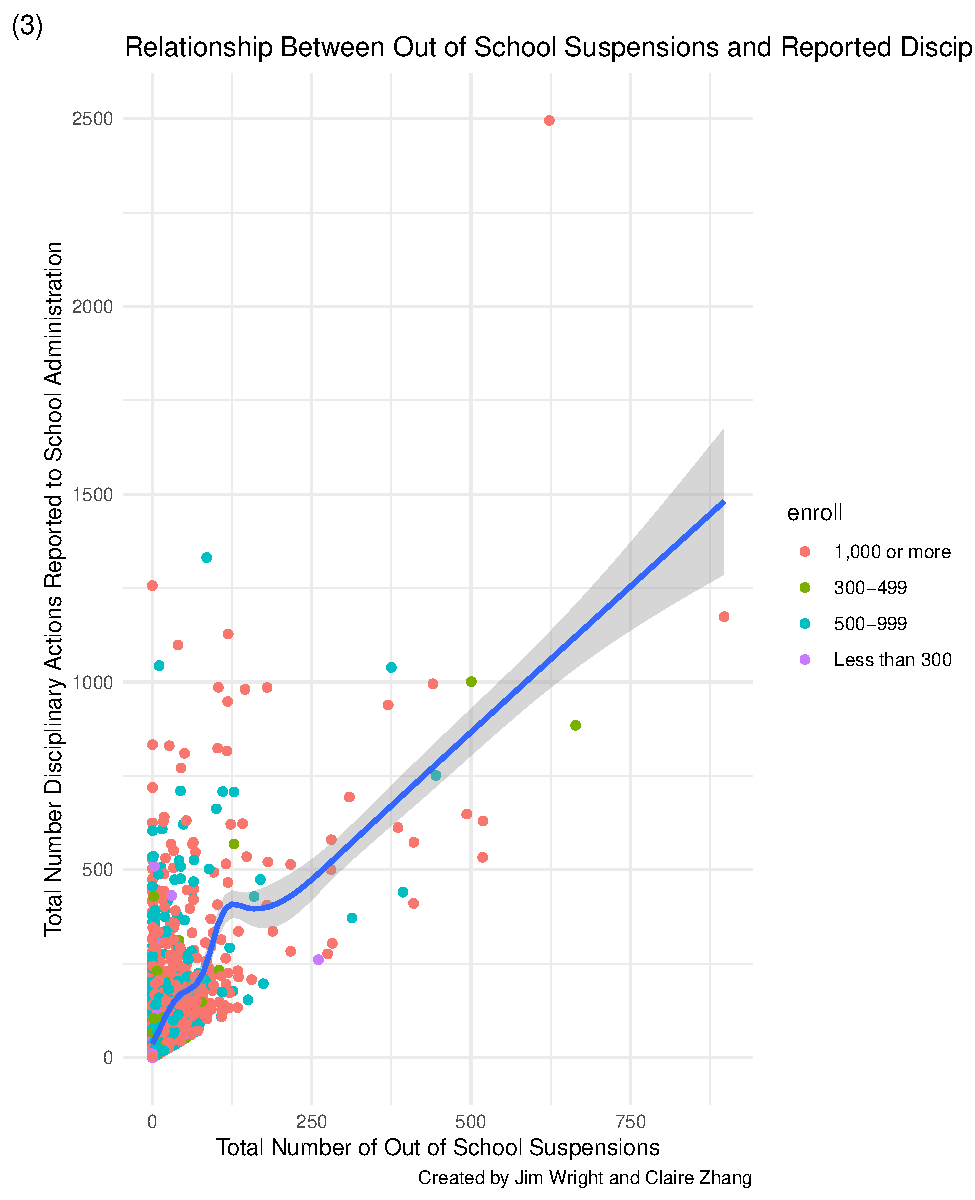
\includegraphics{Final-Project_Zhang_Wright_files/figure-latex/plots-3.pdf}
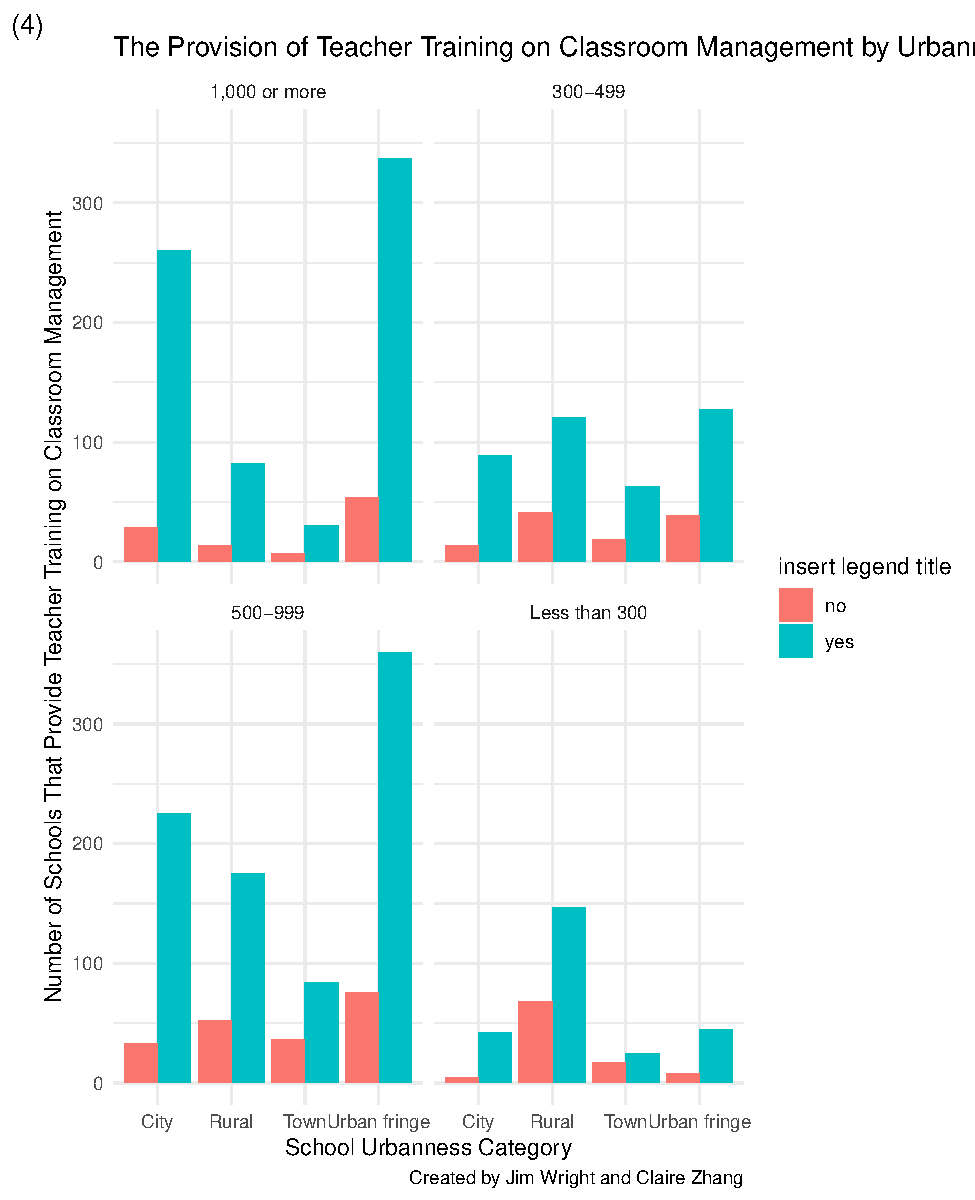
\includegraphics{Final-Project_Zhang_Wright_files/figure-latex/plots-4.pdf}

\begin{verbatim}
## 
## Call:
## lm(formula = oss ~ urban + enroll, data = safe_organized)
## 
## Residuals:
##    Min     1Q Median     3Q    Max 
## -36.03 -10.65  -6.03  -1.02 865.59 
## 
## Coefficients:
##                     Estimate Std. Error t value Pr(>|t|)    
## (Intercept)           36.026      2.045  17.618   <2e-16 ***
## urbanRural            -6.260      2.526  -2.478   0.0133 *  
## urbanTown             -4.338      3.222  -1.346   0.1783    
## urbanUrban fringe     -4.615      2.193  -2.104   0.0354 *  
## enroll300-499        -25.379      2.598  -9.769   <2e-16 ***
## enroll500-999        -21.396      2.125 -10.071   <2e-16 ***
## enrollLess than 300  -28.612      3.055  -9.366   <2e-16 ***
## ---
## Signif. codes:  0 '***' 0.001 '**' 0.01 '*' 0.05 '.' 0.1 ' ' 1
## 
## Residual standard error: 44.8 on 2717 degrees of freedom
## Multiple R-squared:  0.0659, Adjusted R-squared:  0.06384 
## F-statistic: 31.95 on 6 and 2717 DF,  p-value: < 2.2e-16
\end{verbatim}

\begin{figure}
\centering
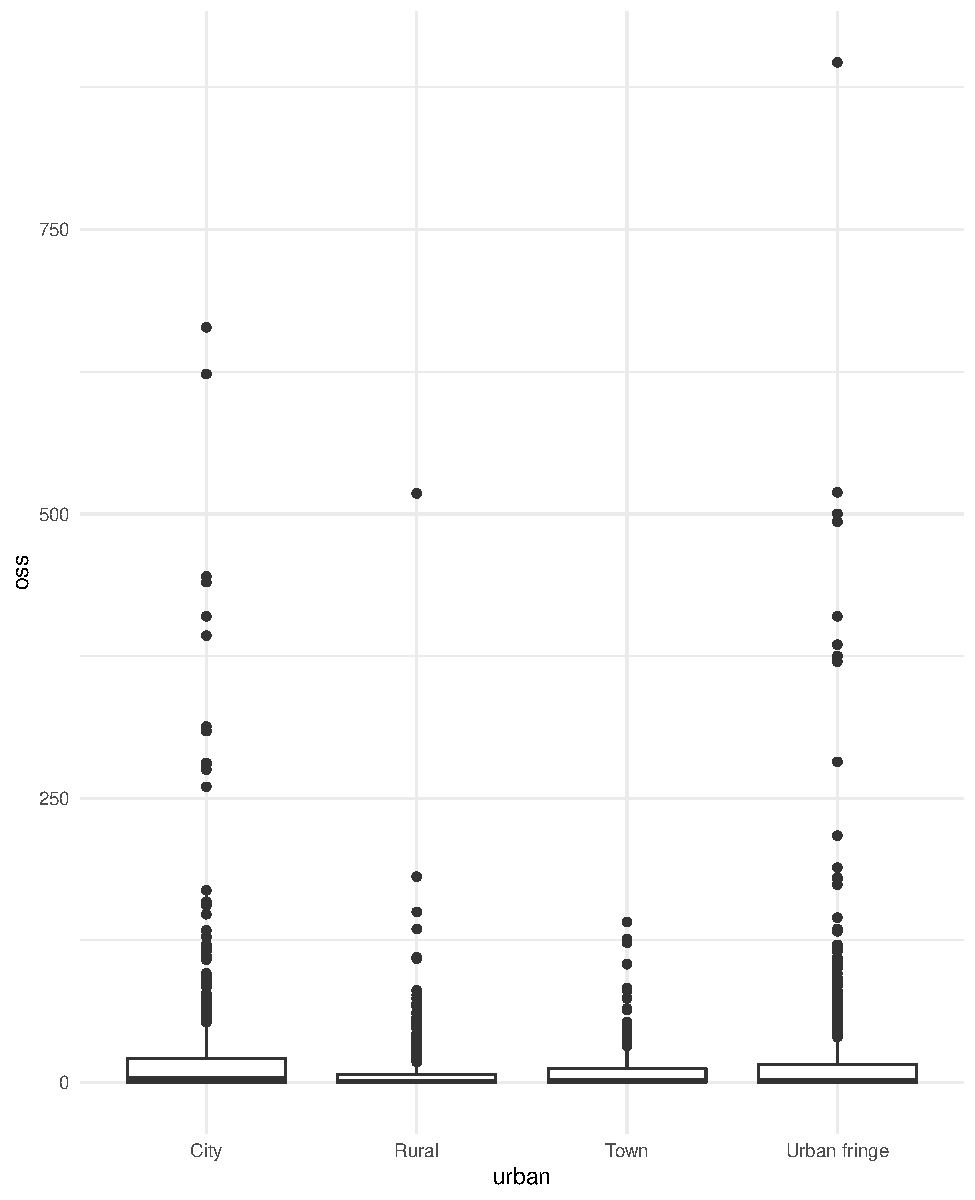
\includegraphics{Final-Project_Zhang_Wright_files/figure-latex/model-1.pdf}
\caption{}
\end{figure}

\begin{verbatim}
## # A tibble: 4 x 2
##   urban        total_oss
##   <chr>            <dbl>
## 1 City             15631
## 2 Rural             5716
## 3 Town              3054
## 4 Urban fringe     17798
\end{verbatim}

\section{Methods}\label{methods}

We report how we determined our sample size, all data exclusions (if
any), all manipulations, and all measures in the study.

\subsection{Participants}\label{participants}

\subsection{Material}\label{material}

\subsection{Procedure}\label{procedure}

\subsection{Data analysis}\label{data-analysis}

We used R (Version 3.6.1; R Core Team, 2019) for all our analyses.

\section{Results}\label{results}

\section{Discussion}\label{discussion}

\newpage

\section{References}\label{references}

\begingroup
\setlength{\parindent}{-0.5in} \setlength{\leftskip}{0.5in}

\hypertarget{refs}{}
\hypertarget{ref-R-base}{}
R Core Team. (2019). \emph{R: A language and environment for statistical
computing}. Vienna, Austria: R Foundation for Statistical Computing.
Retrieved from \url{https://www.R-project.org/}

\endgroup


\end{document}
